\documentclass[conference]{IEEEtran}

\usepackage{amsmath}
\usepackage{amssymb}
\usepackage{booktabs}
\usepackage{graphicx}
\usepackage{tikz}
\usetikzlibrary{arrows.meta, positioning}
\usepackage[hidelinks]{hyperref}

\title{Psychological Markers of Isolation and Emotional Attachment among Students in Long-Term Interaction with AI Companions: A Content Analysis}

\author{
  \IEEEauthorblockN{Anna Merkulova and Adilet Bolat}
  \IEEEauthorblockA{Narxoz University, SCOM3001\\
    Almaty, Kazakhstan\\
    anna.merkulova@narxoz.kz, adilet.bolat@narxoz.kz}
}

\begin{document}
\maketitle



\begin{abstract}
Conversational AI companions are increasingly used for
social interaction and emotional support, raising questions
about emotional attachment and possible social withdrawal.
This paper presents a mixed-methods content-analysis
framework for examining textual indicators of emotional
dependence and social avoidance in student accounts of
interactions with AI companions.

The proposed framework combines qualitative coding,
word-normalized marker frequencies, non-parametric
statistical tests, and regression analysis. It addresses
two research questions: whether emotional-dependence
markers differ across interaction-duration groups (RQ2),
and whether interaction duration is associated with
social-avoidance indicators (RQ3).

To verify the computational workflow, we analyzed
171 synthetic observations. The RQ2 pipeline produced
differences in emotional-dependence marker frequencies
between short- and long-duration groups, with a
Cliff's delta of 0.440. For RQ3, the synthetic data
produced a weak positive Spearman correlation
($\rho=0.136$), whereas the adjusted ordinary least
squares model did not identify a statistically
significant duration coefficient ($p=0.645$).

These numerical results validate the operation of
the analytical pipeline rather than establish
psychological findings about real students.
The study contributes a structured coding approach,
explicit statistical procedures, and a reproducible
research design. Future work will involve ethically
collected authentic data, author-level aggregation,
independent coding, and reliability assessment.
\end{abstract}



\begin{IEEEkeywords}
AI companions, content analysis, emotional attachment, social isolation,
research design
\end{IEEEkeywords}

\section{Introduction}
\label{sec:introduction}

Conversational AI companions are increasingly used in social and emotionally
oriented interactions. Prior research reports that users may turn to these
systems in response to loneliness and may perceive them as sources of social
support~\cite{defreitasAICompanionsReduce2024,maplesLonelinessSuicideMitigation2024}.
Studies have also examined how humanlike qualities, trust, and perceived
consciousness shape users' relationships with conversational systems~
\cite{seymourExploringInteractionsTrust2021,
guingrichAscribingConsciousnessArtificial2024}.


Research on social chatbots has also examined
friendship formation, self-disclosure, and
relationship development over time~
\cite{croesFriendMitsuku2021,
skjuveChatbotCompanion2021,
skjuveLongitudinalRelationships2022,
skjuveAIFriend2022}.


Longitudinal and qualitative studies describe relationship formation with
social chatbots, while also documenting variation in how users experience
and sustain these relationships~\cite{croesFriendMitsuku2021,
skjuveLongitudinalRelationships2022,skjuveAIFriend2022}. This motivates
examining specific interaction markers and reported duration rather than
assuming that AI companionship has one consistent social effect.

The gap addressed by this project is operational: its research questions
connect author-level, word-normalized emotional-dependence markers with
reported use duration and a separately defined isolation--avoidance index.
This design makes the proposed measures and comparisons explicit while
keeping them distinct from causal claims.

The present project addresses this need through a content-analysis design
focused on student accounts concerning Replika and Character.AI. It asks
whether the frequency of emotional-dependence markers differs between users
reporting less than one month and more than three months of use (RQ2), and
whether reported duration is positively associated with an isolation--
avoidance index (RQ3). The analysis is observational; any association will
not establish a causal effect. The repository's current numerical dataset is
synthetic and serves only to test the computational pipeline.

Research on romantic relationships with
social chatbots further illustrates the
diversity of meanings users attribute
to human--AI relationships~
\cite{panMouRomanticRelationships2024}.


The main contributions of this work are:
\begin{itemize}
  \item A structured content-analysis framework
        for identifying attachment, fear-of-loss,
        daily-support, and social-avoidance markers
        in AI-companion interaction accounts.
  \item A mathematical formulation of normalized
        emotional-dependence and social-avoidance
        measures at the author level.
  \item A reproducible statistical analysis plan
        combining non-parametric group comparisons,
        effect-size estimation, correlation analysis,
        and adjusted regression.
  \item A synthetic-data validation of the
        computational pipeline, explicitly separated
        from future empirical investigation
        involving authentic student accounts.
\end{itemize}



The remainder of this paper is organized as follows.
Section~\ref{sec:methodology} presents the research
methodology and mathematical formulation.
Section~\ref{sec:results} reports the synthetic
pipeline-validation results.
Section~\ref{sec:discussion} discusses their
interpretation and threats to validity.
Section~\ref{sec:conclusion} summarizes the
contributions and outlines future research.

\section{Methodology}
\label{sec:methodology}

\subsection{Study design and unit of analysis}
\label{subsec:design}

The planned study uses mixed methods: qualitative content analysis with a
frozen codebook, followed by non-parametric analysis of marker frequencies.
The target corpus consists of English-language user accounts concerning
Replika or Character.AI. The intended unit of analysis is the author, with
markers and word counts pooled across that author's posts before
normalization. The current synthetic test data do not contain author IDs;
therefore, treating one row as one author is a pipeline-test assumption and
must not be carried over as an empirical sampling fact.

\subsection{Measures and formalization}
\label{subsec:measures}

For author $i$, let $w_{ij}$ be the word count for post $j$ and let
$m_{ij}^{(k)}$ be the coded count for dependence marker $k$. Equation~
\ref{eq:dependence-rate} defines the planned emotional-dependence rate per
1,000 words:
\begin{equation}
  F_i = 1000\,
  \frac{\displaystyle\sum_{j=1}^{J_i}\sum_{k\in\mathcal{K}_F}m_{ij}^{(k)}}
       {\displaystyle\sum_{j=1}^{J_i}w_{ij}},
  \label{eq:dependence-rate}
\end{equation}
where $\mathcal{K}_F$ contains attachment, fear-of-loss, and daily-support
markers. For social-avoidance counts $a_{ij}$, the corresponding index is
defined in Equation~\ref{eq:isolation-index}:
\begin{equation}
  I_i = 1000\,
  \frac{\displaystyle\sum_{j=1}^{J_i}a_{ij}}
       {\displaystyle\sum_{j=1}^{J_i}w_{ij}}.
  \label{eq:isolation-index}
\end{equation}

Equations~\eqref{eq:dependence-rate}
and~\eqref{eq:isolation-index} define the
planned author-level rates. The marker
composition is specified in
\texttt{configs/study.yaml} and remains
subject to confirmation before analysis
of authentic data.

\subsection{Collection, coding, and analysis workflow}
\label{subsec:workflow}

The planned workflow is summarized in Fig.~\ref{fig:workflow}. The repository
configuration specifies a minimum post length of 100 words and other quality
filters. 
A second coder is planned for a random
10--20\% subsample, with Cohen's
$\kappa\geq 0.60$ as a preliminary
reliability target. Coding agreement will
be evaluated following established
content-analysis reliability principles~
\cite{krippendorffReliability2004}.
Disagreements will prompt codebook review.
For RQ2, the primary contrast is a one-sided Mann--Whitney
$U$ test between the less-than-one-month and more-than-three-month groups,
with Cliff's $\delta$ and a bootstrap 95\% confidence interval. Kruskal--
Wallis and Jonckheere--Terpstra tests are specified for secondary group and
trend analyses. For RQ3, the plan uses Spearman rank correlation and an OLS
model controlling for weekly session frequency, specified in
Equation~\ref{eq:rq3-model}:
\begin{equation}
  I_i = \beta_0 + \beta_1\,\mathrm{duration}_i
      + \beta_2\,\mathrm{sessions}_i + \varepsilon_i.
  \label{eq:rq3-model}
\end{equation}
The study is cross-sectional and observational, so results will be
interpreted as associations only.


\begin{figure}[t]
  \centering
  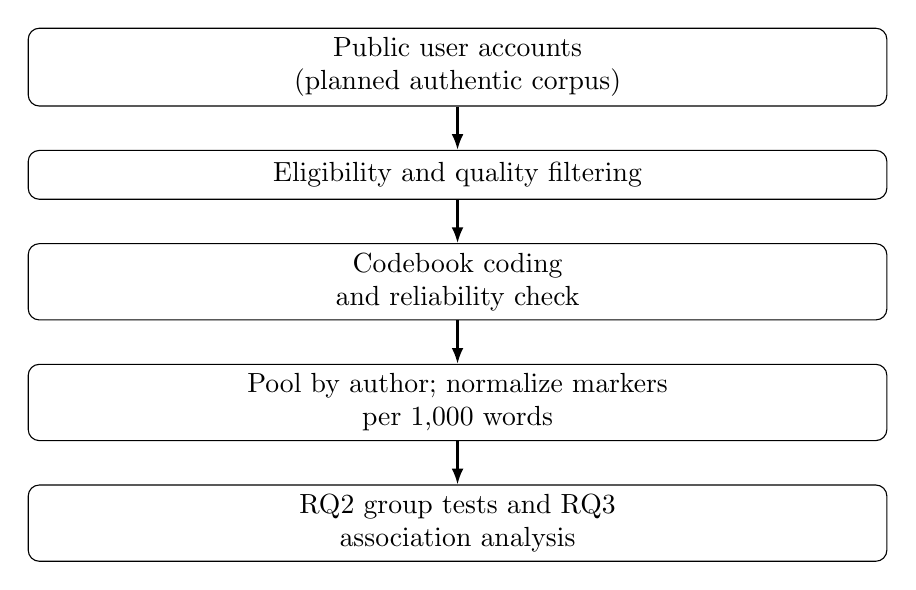
\begin{tikzpicture}[
    node distance=0.55cm,
    stage/.style={draw, rounded corners, align=center,
      text width=0.88\columnwidth, minimum height=0.62cm},
    flow/.style={-{Latex[length=2mm]}, thick}
  ]
    \node[stage] (corpus) {Public user accounts\\(planned authentic corpus)};
    \node[stage, below=of corpus] (filter) {Eligibility and quality filtering};
    \node[stage, below=of filter] (coding) {Codebook coding\\and reliability check};
    \node[stage, below=of coding] (rates) {Pool by author; normalize markers\\per 1,000 words};
    \node[stage, below=of rates] (tests) {RQ2 group tests and RQ3\\association analysis};
    \draw[flow] (corpus) -- (filter);
    \draw[flow] (filter) -- (coding);
    \draw[flow] (coding) -- (rates);
    \draw[flow] (rates) -- (tests);
  \end{tikzpicture}
  \caption{Planned content-analysis workflow. Synthetic repository data are
  used to validate code and do not instantiate the planned human corpus.}
  \label{fig:workflow}
\end{figure}

The project repository also contains synthetic benchmark experiments for
software performance. Those engineering measurements are separate from the
behavioral research questions and are not included in the analysis described
above.


\section{Results}
\label{sec:results}

\subsection{Data Status}

All results reported in this section were generated using
synthetic data for pipeline validation. They do not constitute
empirical evidence about students or AI-companion users.
The synthetic dataset contains 171 observations.

\subsection{RQ2: Emotional-Dependence Marker Frequency}
\label{subsec:rq2-results}

Table~\ref{tab:rq2-summary} summarizes the synthetic
emotional-dependence marker frequencies across three
engagement-duration groups.

\begin{table}[t]
\centering
\caption{Synthetic RQ2 Group Summary (Pipeline Test Only)}
\label{tab:rq2-summary}
\begin{tabular}{lrrr}
\toprule
Duration & $n$ & Median & IQR \\
\midrule
$<1$ month   & 38 & 10.69 & 9.58 \\
1--3 months  & 57 & 11.70 & 12.02 \\
$>3$ months  & 76 & 20.78 & 23.93 \\
\bottomrule
\end{tabular}
\end{table}

The highest median was observed in the synthetic
long-duration group ($>3$ months).

Figure~\ref{fig:rq2-boxplot} displays the synthetic
author-level distributions behind this comparison.


\begin{figure}[t]
  \centering
  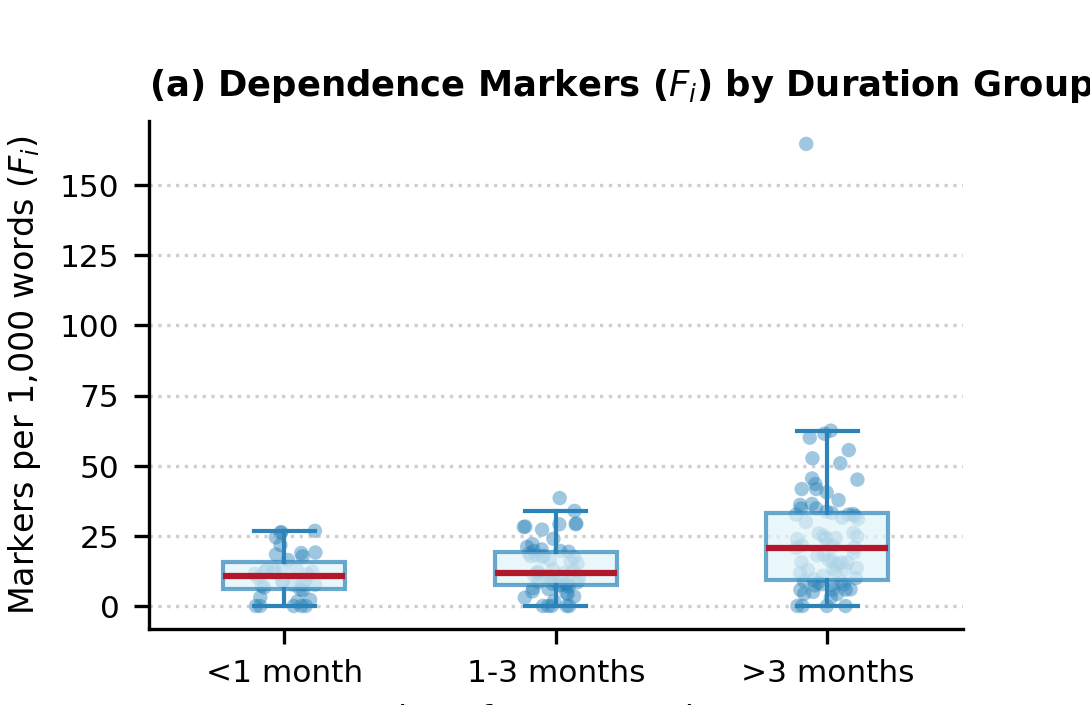
\includegraphics[width=\columnwidth]
    {figures/rq2_boxplot.png}
  \caption{Synthetic emotional-dependence marker
  rates by engagement duration.
  Pipeline validation only.}
  \label{fig:rq2-boxplot}
\end{figure}


The one-sided Mann--Whitney $U$ test comparing the
long-duration and short-duration groups yielded
$U=2079.5$ and $p<0.001$.
Cliff's $\delta$ was 0.440, with a bootstrap
95\% confidence interval of [0.250, 0.614].

The Kruskal--Wallis test across the three groups
yielded $H=19.147$ ($p<0.001$).
The Jonckheere--Terpstra trend test produced
a statistic of 6206.5 ($Z=4.354$, $p<0.001$).

These statistics demonstrate the behavior of the
analysis pipeline on synthetic inputs rather than
substantive findings about human behavior.

\subsection{RQ3: Social-Avoidance Indicators}
\label{subsec:rq3-results}

In the synthetic dataset, Spearman's rank correlation
between engagement duration and the social-avoidance
index was $\rho=0.136$ ($p=0.038$, one-sided).

The correlation between weekly session frequency and
the social-avoidance index was $\rho=0.082$
($p=0.144$, one-sided).

In the OLS model specified in
Eq.~\eqref{eq:rq3-model}, controlling for weekly
session frequency, the duration coefficient was
$\beta_1=-0.129$ ($p=0.645$), while the
session-frequency coefficient was
$\beta_2=-0.619$ ($p=0.278$).

The model explained approximately 0.8\% of the
variation in the synthetic outcome
($R^2=0.008$).

Table~\ref{tab:baseline-comparison} compares
the unadjusted correlation baseline with the
covariate-adjusted analysis on the same
synthetic observations. The coefficients
represent different estimands and are not
directly comparable.

\begin{table}[t]
\centering
\caption{Synthetic RQ3 Baseline Comparison}
\label{tab:baseline-comparison}
\begin{tabular}{lcc}
\toprule
Metric & Spearman & Adjusted OLS \\
\midrule
Duration effect & $\rho=0.136$ & $\beta=-0.129$ \\
$p$-value & 0.038 & 0.645 \\
Controls sessions & No & Yes \\
Observations & 171 & 171 \\
\bottomrule
\end{tabular}
\end{table}


Thus, the weak positive unadjusted correlation
was not reflected in a statistically significant
adjusted duration coefficient.
No substantive inference about real users
can be drawn from these synthetic results.


\section{Discussion}
\label{sec:discussion}

\subsection{Interpretation of RQ2}
\label{subsec:discussion-rq2}

The synthetic RQ2 analysis produced higher
emotional-dependence marker frequencies in the
long-duration group than in the short-duration group,
as shown in Table~\ref{tab:rq2-summary}.

The Mann--Whitney test, Cliff's delta, and the
trend test identified differences in the generated
data. This demonstrates that the analytical pipeline
can compute group comparisons, effect sizes, and
confidence intervals.

However, these patterns originate from synthetic
inputs and cannot establish an association between
AI-companion use and emotional dependence among
real students.

\subsection{Interpretation of RQ3}
\label{subsec:discussion-rq3}

The synthetic RQ3 analysis produced a weak positive
Spearman correlation between interaction duration
and the social-avoidance index.

However, the adjusted OLS duration coefficient was
not statistically significant, and the model explained
less than 1\% of the outcome variation
($R^2=0.008$).

Spearman correlation measures rank-based association,
whereas the OLS coefficient estimates a conditional
linear relationship after accounting for the included
covariate. Their different results may reflect the
distinct statistical quantities being estimated.

These findings demonstrate the importance of
distinguishing statistical significance from
effect magnitude and practical relevance.

\subsection{Relation to Prior Research}
\label{subsec:prior-research}

Previous studies have investigated AI companions
in relation to loneliness and perceived emotional
support~\cite{defreitasAICompanionsReduce2024,
maplesLonelinessSuicideMitigation2024}.

Other research has examined anthropomorphism,
trust, and relationship development in interactions
with conversational technologies~
\cite{seymourExploringInteractionsTrust2021}.

These studies provide a theoretical context for
investigating emotional-attachment and social-avoidance
markers. However, synthetic pipeline results cannot
confirm or contradict empirical findings about
human participants.

\subsection{Limitations and Threats to Validity}
\label{subsec:limitations}

\textbf{Internal validity.}
The synthetic dataset lacks author identifiers.
Treating each observation as an independent author
is therefore a pipeline-testing assumption rather
than a verified sampling property. Human coding
reliability has not yet been established.

\textbf{External validity.}
The planned authentic study focuses on English-language
accounts concerning Replika and Character.AI.
Its future findings may not generalize to other
platforms, languages, or populations.

\textbf{Construct validity.}
Normalized textual marker frequencies are indirect
indicators of emotional attachment and social
avoidance. They cannot establish psychological
diagnoses or fully represent these constructs.

\textbf{Causal limitations.}
The proposed study is observational and
cross-sectional. Statistical associations would
not establish causal effects of AI-companion use.

\textbf{Data status.}
The current results validate computational
procedures only. Empirical conclusions require
authentic data, documented ethical safeguards,
verified sampling units, and independent coding
reliability assessment.


\section{Conclusion and Future Work}
\label{sec:conclusion}

This paper presents a mixed-methods research framework
for investigating textual markers of emotional attachment
and social isolation in accounts of interaction with
AI companions. The framework combines qualitative
content analysis, normalized marker frequencies,
non-parametric statistical tests, and regression analysis.

For RQ2, the synthetic pipeline test produced higher
emotional-dependence marker frequencies in the
long-duration group than in the short-duration group.
The statistical procedures successfully generated
group comparisons, effect-size estimates, and
confidence intervals. These results demonstrate
pipeline functionality but do not constitute
empirical evidence about human behavior.

For RQ3, the synthetic data yielded a weak positive
Spearman correlation between engagement duration
and social-avoidance indicators. However, the adjusted
OLS model did not produce a statistically significant
duration coefficient and explained less than 1\%
of the outcome variation. These findings illustrate
the importance of comparing statistical approaches
and interpreting their results cautiously.

Future work will focus on three priorities.
First, an authentic corpus will be collected and
analyzed with documented ethical and privacy safeguards.
Second, author-level aggregation and coding reliability
will be verified using the planned codebook and
independent coders. Third, the analysis will be
extended to additional platforms and populations,
with sensitivity analyses to evaluate the robustness
of the observed associations.

Overall, the current contribution is a reproducible
research design and a tested analytical workflow,
rather than confirmed psychological findings
about AI-companion users.


\bibliographystyle{IEEEtran}
\bibliography{references}
\end{document}
